\documentclass[times, utf8, diplomski]{fer}
\usepackage{booktabs}
\usepackage[utf8]{inputenc}

\usepackage[T1]{fontenc}
\usepackage{fixltx2e}
\usepackage{graphicx}
\usepackage{longtable}
\usepackage{float}
\usepackage{wrapfig}
\usepackage{soul}
\usepackage{textcomp}
\usepackage{marvosym}
\usepackage{wasysym}
\usepackage{latexsym}
\usepackage{amssymb}
\usepackage{hyperref}
\usepackage{caption}
\usepackage{pdfpages}
\usepackage{float}
\usepackage[usenames, dvipsnames]{color}
\usepackage{listings}
\usepackage{xcolor}
\usepackage{subfig}
\usepackage{algpseudocode}
\usepackage[Algoritam]{algorithm}

\lstset { %
    language=C++,
    backgroundcolor=\color{black!5}, % set backgroundcolor
    basicstyle=\footnotesize,% basic font setting
}

\begin{document}

\title{LISA - Alat za poravnanje DNA očitanja}

\author{Filip Paveti\'{c}, Goran \v{Z}u\v{z}i\'{c}}

\maketitle

\newcommand{\zahvalaX}[1]{%
	\newpage
 	\setcounter{page}{3}
	\vspace*{\fill}
	#1
	\vspace*{\fill}
}


% Dodavanje zahvale ili prazne stranice. Ako ne želite dodati zahvalu, naredbu ostavite radi prazne stranice.
\zahvalaX{Ovaj rad izrađen je na Fakultetu elektrotehnike i računarstva Sveučilišta u Zagrebu, na Zavodu \
za elektroničke sustave i obradbu informacija pod vodstvom doc. dr. sc. Mile Šikića i predan je na natječaj \
za dodjelu Rektorove nagrade u akademskoj godini 2012. / 2013.}

\tableofcontents

\chapter{Uvod}
Ovaj rad opisuje sustav za mapiranje DNA sekvenci na referentni genom. Rad je podijeljen na 4 dijela:
\begin{itemize}
\item u prvom dijelu ćemo napraviti kratki uvod u probleme bioinformatike i pozadinu problema kojeg sustav rješava
\item u drugom dijelu se bavimo modelom, algoritmom i implementacijom nad kojim je sustav ostvaren
\item nakon toga prezentiramo rezultate testiranja i usporedba s najpoznatijim analognim alatima
\item naposljetku dajemo kratki zaključak i smjernice za daljnji rad
\end{itemize}

Sustav je razvijen u sklopu natjecanja identifikacija organizama iz toka DNA sekvenci
kojeg je objavila tvrtka \emph{InnoCentive} pod sponzorstvom vlade Sjedinjenih Američkih Država
i koje je u tijeku \footnote{više informacija o samom natjecanju možete pronaći na \emph{http://tinyurl.com/dna-dtra}}.

\section{Bioinformatika}

Bioinformatika je u posljednjih nekoliko godina u centru ogromne pažnje i entuzijazma zbog napredaka u razumijevanju živih bića i brzom razvoju tehnologije pomoću kojih ih možemo proučavati.
Tijekom 20. stoljeća se bioinformatika koristila u svrhe proučavanja nasljednih svojstava, evolucije između vrsta te identifikacije
patogenih bakterija, dok se u bliskoj budućnosti vjeruje kako će pomoći u proizvodnji boljih lijekova koji bi bili
posebno prilagođeni zaraženoj osobi.

Molekularna biologija i biokemija su nam otkrili kako najveću funkcionalnu ulogu u gotovo svim biološkim procesima
živih organizama imaju molekule zvane \emph{proteini}, linearni nizovi aminokiselina spojenih peptidnim vezama.
Njihova uloga u organizmima seže od katalizacijskih procesa (npr. kod metabolizma), signalizacije i adhezije stanica
sve do imunološkog sustava. Proteini su konstruirani zasebno u svakoj stanici od svojih gradivnih elemenata (aminokiselina) prema uputstvu zapisanim u masivnoj staničnoj molekuli
deoksiribonukleinske kiseline (DNA).

Dominantno područje bioinformatike se bavi sekvenciranjem (čitanjem) i analizom DNA, koja je po svojoj strukturi dugi linearni niz sastavljen od otprilike
3 milijarde\footnote{kod ljudi} povezanih parova baza nukleinskih kiselina. Masivnost tih brojeva stvara potrebu za razvojem računalnih alata
bez kojih bilo kakva obrada postaje nemoguća.

Nedavni je razvoj moderne tehnologije doveo do strmoglavog pada cijene sekvenciranja molekule DNA do te razine da je
postalo jasno kako će u bliskoj budućnosti najsporiji i najteži dio bioinformatike biti u konstrukciji efikasnih
algoritama koji brzo i pouzdano obrađuju rastuću količinu informacija na njihovom raspolaganju.

\section{DNA i mutacije}
Kao što je spomenuto, DNA modeliramo kao linearni niz povezanih parova baza. U DNA se pojavljuju točno četiri različite baze i njih
označavamo slovima \emph{A, G, T} i \emph{C}\footnote{skraćeno od adenin, guanin, timin i citozin, vrsta nukleinskih kiselina koje se pojavljuju}.
Tako DNA reprezentiramo dugim nizom slova nad gornjom četvoroslovnom abecedom, primjerice:

\begin{verbatim}
... AGTGAGGAAAAAAAAAGGTCAATGCAGCACTTGAGCCAACATTGTAGAT
    GTTGTACTGCAAGGTCAGGTCTCGCCCCTCCACGGCGTATCTGTTCAG
    CAGTGACTTGGAGGCAAGAAAATCAAACCCGTGATCGATGGTACCGAGC ...
\end{verbatim}

Kroz vrijeme se na molekuli DNA javljaju razne mutacije. Okvirno poznavanje mogućih mutacija je nužno za bolje razumijevanje izazova koji se javljaju u bioinformatici. Biolozi su izolirali nekoliko dominantnih vrsta:

\begin{enumerate}
\item Supstitucija - zamjena jedne baze drugom. Najčešća mutacija.
  Uzrokovana greškama u replikaciji i kemikalijama.
  \nopagebreak
  \begin{figure}[!ht]
    \begin{center}
      A C G \textcolor{blue}{T} T G A C \\
      A C G \textcolor{red}{A} T G A C
      \caption{Primjer supstitucije}
    \end{center}
  \end{figure}

\item Ispuštanje i umetanje - iz DNA se ukloni ili doda slijed baza. Ova mutacija je vrlo štetna i obično
  rezultira gubitkom funkcionalnosti dijela gena.

  \nopagebreak
  \begin{figure}[!ht]
    \begin{center}
      A C G \textcolor{red}{T T G} A C \\
      A C G A C
      \caption{Primjer ispuštanja}
    \end{center}
  \end{figure}
\item Udvostručavanje - ponavljanje dijela sekvence dva ili više puta zaredom. Ova mutacija je iznimno rijetka,
  ali se smatra da je unatoč tomu imala veliku ulogu u povećanju genetskog koda živih bića.
  \begin{figure}[!ht]
    \begin{center}
      A C G \textcolor{blue}{T T G A} C \\
      A C G \underline{\textcolor{red}{T T G A}} \underline{\textcolor{red}{T T G A}} C \\
      \caption{Primjer udvostručavanja}
    \end{center}
  \end{figure}
  
\item Inverzija - okretanje dijela sekvence. Iznimno rijetka mutacija koja se najčešće zanemaruje pri analizi.
  \begin{figure}[!ht]
    \begin{center}
      A C \textcolor{blue}{T C A A} G G \\
      A C \textcolor{red} {A A C T} G G
      \caption{Primjer inverzije}
    \end{center}
\end{figure}
\end{enumerate}

\section{Sekvenciranje DNA}

Prvi pokušaj sekvenciranja ljudskog DNA počinje 1990. američkim \emph{Human Genome Project}-om koji je trajao 15
godina i uspješno identificirao većinu ljudskog genoma. Ukupna cijena projekta je procijenjena na 3.000.000.000\$.
\cite{genomefaq}
Od tada cijena sekvenciranja DNA strmoglavo pada i očekuje se će u sljedećih nekoliko godina dostići 1.000\$ za
cjelokupni ljudski genom.

Sekvenciranje DNA se odvija u nekoliko faza: (1) prikupljanje kratkih očitanja, (2) poravnavanje s referentnim genomom, (3) izlistavanje varijanti i (4) filtriranje i označavanje. \cite{mardis2008next}

\begin{description}
\item[Prikupljanje kratkih očitanja] je biološki dio sekvenciranja tijekom kojeg se DNA višestruko replicira, slučajno lomi na dijelove duljine 100-3000 baza te se potom očitava složenim metodama. Te metode su podložne pogreškama uslijed krivog očitanja dijela sekvenci, gubljenja informacija i dvosmislenosti podataka koji se javljaju tijekom loma.

\item[Poravnavanje s referentnim genomom] je proces mapiranja očitanih fragmenata na referentni genom. Uobičajeni volumen podataka od otprilike desetke milijuna očitanja i tri milijarde startnih pozicija čini ovaj posao vrlo
algoritamski zahtjevnim. Još kritičnijim ovaj korak čini svojstvo da se sve greške na ovom koraku propagiraju i
ruše kvalitetu svim preostalim dijelovima sekvenciranja.

\item [Izlistavanje varijanti] je korak u kojem se uspoređuju poravnata očitanja s referentnim genomom. Pronađene
mutacije mogu biti uzročnici nasljednih bolesti ili mogu jednostavno biti genski šum bez funkcionalnih svojstava.

\item [Filtriranje i označavanje] procjenjuje koja od potencijalnih razlika između interesantnih gena pridonosi 
patološkom procesu kojeg proučavamo. Filtriraju se mutacije bez funkcionalnih značajki te se prepoznaju česte populacijske mutacije.
\end{description}

\section{Obrazloženje teme}

Izgrađeni sustav se bavi problematikom \emph{poravnavanja očitanja s referentnim genomom}. Specifično, potrebno
je za svaki od nekoliko desetaka milijuna očitanja koja su skupljena u FASTQ datoteku mapirati na poziciju u
referentnom genomu. Problem su pritom gore opisane mutacije, pogreške u kratkim očitanjima, dvosmisleni podaci,
regije niske složenosti te repetitivne regije koje se mogu mapirati na više mjesta u referentnom genomu.

Ovaj sustav se koristi kao prvi korak prilikom rješavanja problema identifikacije organizama iz toka DNA sekvenci
koji se pojavio na natjecanju \emph{Innocentive}. Autori ovog rada sudjeluju
na tome natjecanju u sklopu tima Fakulteta elektrotehnike i računarstva Sveučilišta u Zagrebu.




\chapter{Pristup}

\section{Pregled postojećih rješenja}
Ovo poglavlje počinjemo kratkih pregledom trendova u razvoju mappera te kasnije dajemo detaljan opis našeg pristupa. Jedan od prvih algoritama za poravnanje očitanja je algoritam globalnog poravnanja pod nazivom Smith-Waterman\cite{Smith1981195}. Rješenje dobiveno tim algoritmom može se smatrati veoma točnim zbog toga što ima statistički opravdano značenje, međutim zbog velike vremenske složenosti algoritma nije praktično za korištenje.\\
Većina boljih modernih alata za mapiranje - \emph{mappera} (poput SNAP-a\cite{SNAP} i SeqAlto-a\cite{seqalto}) koriste \emph{seed-and-extend} pristup. U tom pristupu prvo se od 
referentnog genoma gradi indeks koji mapira niz od svakih uzastopnih k-znakova genoma na sve pozicije unutar genoma na kojima se taj podniz nalazi. Ukupan broj takvih različitih podnizova je $4^k$, što je i prva praktična opaska, jer za $k\le32$ možemo takav podniz zakodirati u $64$-bitni cjelobrojni tip podataka. Očitanja se obrađuju na način da se ponovno promatraju podnizi uzastopnih znakova duljine $k$ te se vrši upit u prethodno izgrađeni indeks. Pozicije dobivene takvim upitom daju kandidatne pozicije u čijoj se okolini nalazi potencijalno poravnanje očitanja na genom. Razlike između mappera ovog tipa su primarno u načinu izgradnje indeksa i načinu ocjene kvalitete poravnanja na nekoj kandidatnoj poziciji. Tako primjerice SNAP koristi tablicu raspršenog adresiranja kao strukturu podataka nad kojom je izgrađen indeks, dok SeqAlto koristi sortirano polje. Za ocjenu kvalitete SNAP koristi \emph{edit-distance} metriku, dok SeqAlto koristi općenitiju \emph{Needleman-Wunsch}\cite{nw} metriku. Oba pristupa daju značajno poboljšanje efikasnosti u odnosu na pristup spomenut na početku ove sekcije, međutim ti su mapperi i dalje nepraktični budući da kroz vrijeme strojevi za izradu očitanja napreduju i duljine očitanja postaju sve veće čime pretpostavke koje osiguravaju efikasnost ovih alata postaju prejake (glavni razlog je što u njihovim implementacijama izračun tih metrika ima vremensku složenost linearno proporcionalno s duljinama očitanja).\\
Naš mapper indeks izgrađuje po uzoru na SeqAlto, međutim uvodimo novu metriku ocjene kvalitete koja za red složenosti poboljšava postojeće algoritme bez gubitka točnosti što ćemo potkrijepiti eksperimentima u kasnijim poglavljima.
Metrika kvalitete bazira se na traženju najduljeg uzlaznog podniza\footnote{engl. Longest Increasing Subsequence; odatle dolazi inspiracija za naziv LISA - LIS Aligner}\\

\section{Opis pristupa}

Glavna inspiracija prema našem algoritmu proizlazi iz nekoliko svojstava. Prvo, za malu količinu grešaka (koje predstavljaju realan slučaj, očitanja s velikim postotkom greške nisu korisna za ikakve zaključke) unutar očitanja postojat će mnogo nizova uzastopnih znakova koji nisu dotaknuti greškom. Mi želimo iskoristiti tu činjenicu pa dizajniramo algoritam koji nastoji poravnati dijelove netaknute greškom, a one koji je sadrže ignorira. Pokazuje se da je za veće duljine očitanja ovaj pristup iznimno uspješan\footnote{Trenutna pretpostavka koju radimo je da dugačka očitanja imaju svoje jedinstveno mjesto u genomu. Neki drugi mapperi ne rade tu pretpostavku pa je u daljnjim planovima razvoja LISA-e dopustiti mogućnost poravnanja na više različitih mjesta unutar genoma.}
\\
\\

\begin{figure}[H]
\centering
\includegraphics[width=0.9\textwidth]{../img/poravnanje-intuicija.pdf}
\caption{Primjer poravnanja - dobro poravnanje ima jako puno preklapajućih dijelova}\label{poravnanje-intuicija}
\end{figure}

\subsection{Indeks}
U pregledu poglavlja spomenuli smo da za izgradnju indeksa pratimo smjernice SeqAlto mappera. Svaki niz $i$ od $k=20$ uzastopnih znakova na poziciji $p_i$ unutar genoma kodiramo jednim cijelim brojem $h_i$ koji predstavlja hash bez kolizije. Indeks nam čini polje uređenih parova $(h_i, p_i)$. To je polje sortirano pa koristimo binarno pretraživanje kako bi dohvat pozicija za neki zadani hash bio efikasan. Dodatno, one $h_i$-ove koji se pojavljuju jako velik broj puta njihove parove mičemo iz niza jer takvi ne donose korisnu informaciju, a samo povećavaju vremensku i memorijsku složenost. 


\begin{table}[H]
  \centering
  \subfloat[DNA nad kojom gradimo indeks, uz $k=5$]{
    \centering
    \begin{tabular}{|c|c|c|c|c|c|c|c|c|c|c|c|c|c|c|c|c|c|}
      \hline
      A&C&G&T&A&G&A&C&G&T&A&G&A&T&A&G&A&A\\
	\hline
	1&2&3&4&5&6&7&8&9&10&11&12&13&14&15&16&17&18\\
	  \hline
    \end{tabular}
  }
  
  \subfloat[Indeks]{
    \centering
    \begin{tabular}{|c|c|}\hline
ACGTA&1,7\\
\hline
AGACG&5\\
\hline
AGATA&11\\
\hline
ATAGA&13\\
\hline
CGTAG&2,8\\
\hline
GACGT&6\\
\hline
GATAG&12\\
\hline
GTAGA&3,9\\
\hline
TAGAA&14\\
\hline
TAGAC&4\\
\hline
TAGAT&10\\
\hline
    \end{tabular}
  }
  
  \caption{Konceptualni prikaz indeksa}\label{indeks}
\end{table}

\subsection{LISA algoritam poravnanja}
Algoritam poravnanja sastoji se od dva koraka:
\begin{enumerate}
\item Grubo određivanje pozicije očitanja unutar genoma
\item Fino određivanje pozicije očitanja unutar genoma
\end{enumerate}

\subsection{Grubo određivanje pozicije očitanja}

U ovoj osnovnoj fazi algoritma poravnanja određujemo poziciju unutar genoma oko koje je očitanje koncentrirano. Opća ideja iza algoritma je konstrukcija niza brojeva (kojeg ćemo uskoro opisati) nad kojim pokrećemo algoritam nalaženja najduljeg rastućeg podniza\footnote{algoritam je opisan u dodatku}. Nađeni podniz ugrubo opisuje poziciju poravnanja i koristi se u sljedećoj fazi za traženje točne pozicije poravnanja.\\
Potreban niz $P$ konstruiramo tako da promatramo sve nizove uzastopnih znakova $i$ duljine $k$ unutar očitanja s lijeva na desno. Za svaki od njih vršimo upit za pozicije unutar kojih se nalazi u indeksu. Na kraj niza $P$ za svaku od dobivenih pozicija $x$ dodajemo par $(x,i)$. Kada smo to učinili za sve nizove $i$, sortiramo $P$ po prvom broju u paru i pokrećemo algoritam pronalaska najduljeg zajedničkog podniza $L$ nad nizom drugih brojeva parova u $P$. $L$ koristimo u sljedećoj fazi. Pseudokod algoritma dan je u \ref{grubo}.



\begin{algorithm}[H]
\begin{algorithmic}
\State $P \gets \{\}$
\State $L \gets \{\}$
\For{$i=1...duljina(O)-k+1$}
	\ForAll{$p \in dohvatiPozicijeIzIndeksa(O[i...i+k-1])$}
		\State $P \gets P \cup (p, i) $
	\EndFor
	
	\State $P \gets sortirajPoPrvomBroju(P)$
	\State $L \gets najduljiRastuciPodnizPoDrugomBroju(P)$
	\State \Return $L$
\EndFor

\end{algorithmic}
\caption{$GruboPoravnanje(O)$}\label{grubo}
\end{algorithm}


\subsection{Fino određivanje pozicije očitanja}

\begin{figure}[H]
\centering
\includegraphics[width=0.8\textwidth]{../img/fino.pdf}
\caption{Višestruka poravnanja}\label{img:fino}
\end{figure}

Razlog zašto je ova faza potrebna je vidljiv na \ref{img:fino}. Očito je da je pravo poravnanje smješteno oko pozicije 9, dok bismo pogrešnom naivnom procjenom možda rekli da je ono ipak na poziciji 1. Pseudokod \ref{fino} opisuje rad ove faze.

\begin{algorithm}[H]
\begin{algorithmic}
\State $brojac(-\infty...\infty) \gets 0$
\ForAll{$l \in L$}
	\State $++brojac(prvi(l)-drugi(l))$
\EndFor
\State $finaProcjena \gets \arg\max_i brojac(i)$
\State \Return $finaProcjena$
\end{algorithmic}
\caption{$FinoPoravnanje(L)$}\label{fino}
\end{algorithm}


\subsubsection{Mjera pouzdanosti}

Mjerenje pouzdanosti je još uvijek otvoren problem za LISA-u. Trenutno je u uporabi omjer duljine pronađenog rastućeg niza i duljine očitanja.

\chapter{Implementacija}

Sustav je implementiran u programskom jeziku C++ (zbog efikasnosti i ogromnog volumena podataka) koristeći nedavni standard C++0x/C++11 pomoću kompatibilnog GNU g++ prevoditelja.

Implementacija sustava može biti vrlo prirodno razložena na dva osnovna dijela:

\begin{enumerate}
\item izgradnja indeksa nad referentnom bazom gena (potrebno je pripremiti bazu genoma)
\item mapiranje očitanja na referentnu bazu (potrebno je pripremiti datoteku s očitanjima)
\end{enumerate}

Prije bilo kakvog mapiranja potrebno je jednokratno izgraditi indeks, ali je nakon toga moguće neograničeno puta koristiti izgrađeni indeks pri mapiranju podataka, kao što je prikazano na dijagramu:

\begin{figure}[!ht]
\begin{center}
	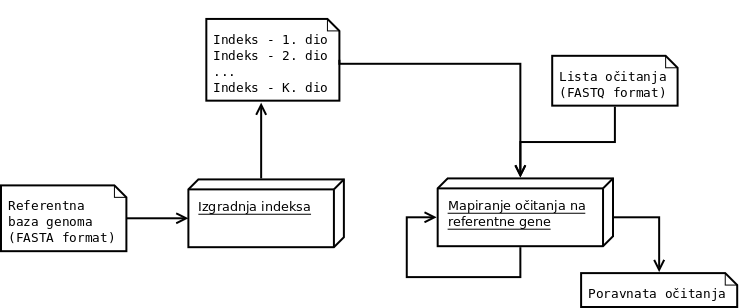
\includegraphics[width=1\textwidth]{../img/Komponente.png}
	\caption{Dijagram komponenata s njihovih ulazima/izlazima}
\end{center}
\end{figure}


Ostatak poglavlja će detaljnije obraditi pojedine komponente opisanog algoritma te njihove ulazne/izlazne podatke.

\section{Priprema podataka}

\section{Izgradnja indeksa}
Zbog iznimnog volumena referentne baze od 47 GB i procijenjene veličine izlaznog indeksa od 340 GB memorije nije
pogodno graditi indeks od cijele baze odjednom. Odabrali smo pristup gdje bazu dijelimo na više jednakih dijelova
(čija se veličina može specificirati preko komandne linije) te gradimo zasebni indeks na svakom od tih dijelova.

Implementacijski gledano, indeks je binarna datoteka koja sadrži sortiranu hash tablicu svih genskih podsekvenci
duljine $N$ nukleotidnih baza\footnote{tipično, uzimamo $N = 16$ ili $N = 20$}. Specifično, svaku podsekvencu
duljine $N$ možemo interpretirati kao broj u bazi 4 te tako dobiveni broj uzimamo kao ključ dotične pozicije koji se sortira i sprema u indeks. Ovakav odabir omogućuje brzo pretraživanje po ključu pomoću logaritamskog binarnog 
pretraživanja. Dodatno, moguće je i pretraživati podsekvence po ključu koji je manji od $N$
iz razloga što za $N < 32$ i 64-bitni tip podataka nema preljeva.

Sama struktura binarne indeks datoteke je najbolje opisana opisnikom pretinaca hash tablice, prikazanim u sljedećem
odsječku:

\begin{lstlisting}
  struct Entry {
    size_t position;
    hash_t hash;

    friend bool operator < (const Entry& a, const Entry& b) {
      return a.hash < b.hash;
    }
  };
\end{lstlisting}

Bitno je napomenuti kako koristimo razne implementacijske i algoritamske optimizacije radi efikasnijeg
baratanja podataka ogromnog volumena s kakvima radimo u ovom projektu. Ovdje ćemo ukratko objasniti neke od njih:

\begin{description}
\item [Paralelno sortiranje pretinaca] se pokazalo kao prirodna optimizacija nakon profiliranja programskog koda.
Ispostavilo se da je upravo ovaj korak najsporiji dio izgradnje indeksa. Za ubrzanje koristimo paralelni stabilni
sort implementiran u OpenMP biblioteci (verzije 1.3).
\item [Micanje podsekvenci s visokom frekvencijom pojavljivanja]. Intuitivno je jasno kako podsekvence s vrlo visokom frekvencijom pojavljivanja (preko 6 redova veličine više od prosjeka) kodiraju repetitive regije ili 
regije niske složenosti i pritome nimalo ne pridonose kvaliteti poravnanja. Kako bismo što smanjili obujam podataka
i ubrzali fazu poravnavanja, sustav izbacuje one podsekvence čija frekvencija pojavljivanja je 5 puta veća od
prosjeka \footnote{postiže se smanjenje količine podataka od oko 15\%}. Kako bismo opravdali takvu redukciju
podataka, analizirali smo frekvenciju pojedinih podsekvenci i potvrdili kako se pojedine jedinke pojavljuju više
redova veličina od prosjeka, kao što je prikazano na sljedećem grafu:

\begin{figure}[!ht]
\begin{center}
	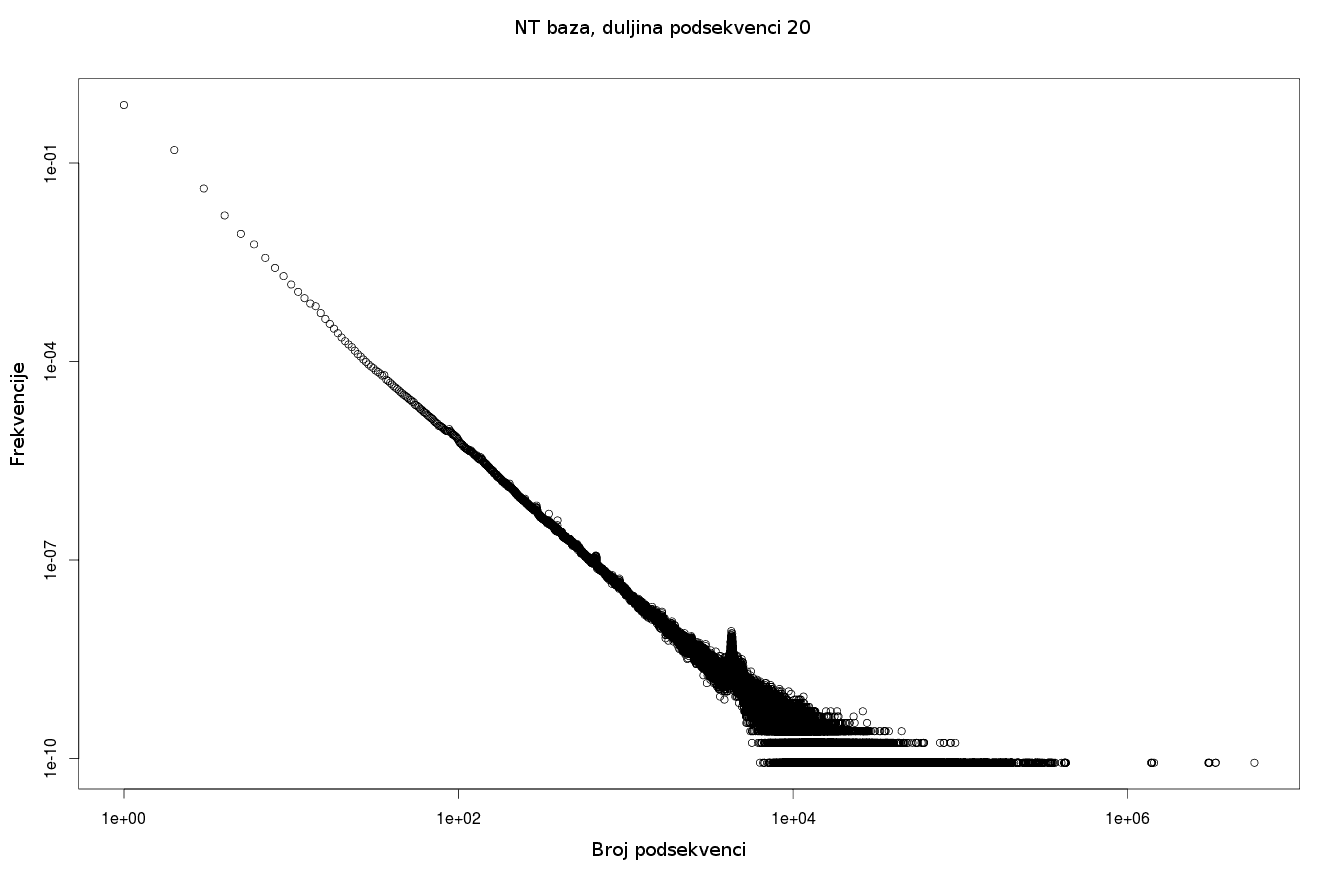
\includegraphics[width=0.9\textwidth]{../img/kmers_20.png}
	\caption{Vrijednost y-ona predstavlja vjerojatnost da se slučajno odabrana podsekvenca u bazi javlja točno x puta.}
\end{center}
\end{figure}

\end{description}

Cjelokupna izgradnja indeksa nakon optimizacija traje otprilike 4 sata računalu performansa 192 GB RAM-a i Intel(R) Xeon(R) procesorom s 12 jezgara koje rade na 2.40 GHz.

\section{Mapiranje očitanja}

Mapiranje očitanja na referentnu bazu zahtjeva izgrađeni dio indeksa koji se u potpunosti učitava u radnu memoriju. Iz ovog razloga je potrebno unaprijed odrediti prihvatljivu veličinu indeksa koju je moguće u potpunosti učitati.

Algoritam mapira pojedino očitanje tako da pokušava pronaći najbolje poravnanje s referentnom bazom. Za svaku
podsekvencu pronalaze se sve pozicije u genima gdje se navedena podsekvenca pojavljuje. Pretraga se, zbog
sortiranosti podataka vrši binarnim pretraživanjem, a može se zbog velike količine podataka i uniformne hash
funkcije ubrzati interpoliranim binarnim pretraživanjem. \cite{weiss1998data}

Za svaki gen u kojem je pronađena barem jedna odgovarajuća podsekvenca se poravnava s fragmentom pomoću opisanog
algoritma najdužeg rastućeg podniza. Implementacija algoritma je ostvarena u složenosti $O(n \log n)$ pomoću
vrlo efikasnog Fenwickovog stabla koje podržava sve potrebne operacije kao i klasično balansirano binarno stablo,
ali uz puno bolju vremensku i memorijsku konstantu. \cite{fenwick1994new}

Kako bi se ubrzao proces mapiranja, očitanja su ravnomjerno podijeljena među jezgrama računala (sustav
automatski detektira broj jezgara i ravnomjerno dijeli posao). Osiguranje ravnomjerne zaposlenosti je ostvareno
korištenjem reda dretvenih zadataka (engl. \emph{ThreadPool}) uz rotirajući binarni semafor (engl. \emph{Spinlock})
kako bi se fragmenti fino granulirali i radi osiguranja što efikasnije sinkronizacije među dretvama. Koristimo
biblioteku \emph{pthreads} kako bi omogućili višedretveno mapiranje.

\section{Distribucija mapiranja}
Veliki volumen podataka prisutan pri rješavanju ovog problema nas je potakao da distribuiramo algoritam na
više računala. Specifično, korisnik pokreće sustav za mapiranje na jednom računalu koje potom dijeli ulaznu 
datoteku očitanih fragmenata na jednake dijelove te ih šalje na farmu servera koji potpuno paralelno obrađuju
dane podatke i pri završetku šalju rezultate natrag na originalno računalo. Distribucija se vrši preko biblioteke
MPI\cite{gabriel04:_open_mpi}, kao što je prikazano na slici:

\begin{figure}[H]
\begin{center}
	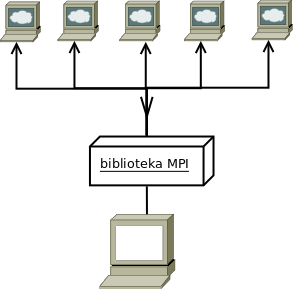
\includegraphics[width=0.45\textwidth]{../img/MPI.png}
	\caption{Distribucija mapiranja na farmu servera}
\end{center}
\end{figure}

Isplativost distribucije mapiranja proizlazi iz fine granularnosti originalnog problema - višestruko se riješava identična zadaća mapiranja fragmenta na referentni genom, što svakoj paralelizaciji na broj računala znatno manji od broja fragmenata osigurava linearno ubrzanje vremena izvršavanja.

\chapter{Rezultati}

\section {Pregled}
U ovoj sekciji analiziramo performanse LISA-e. Analiza se provodi poravnanjem nad poznatim vrstama bakterija - kuga, salmonela, streptokok i E. Coli. Motivacija iza preciznog poravnanja očitanja u genome bakterije je jasna - efikasno i točno određivanje primjerice mutacija omogućuje brži dizajn lijekova za bakterije koje su stekle otpornost na postojeće lijekove.\\
Dajemo usporedbu LISA-e sa nekoliko modernih mappera. Uspoređujemo točnost i brzinu sa BWA-SW, BWA-MEM\cite{Li:2010:FAL:1741823.1741825}, SNAP i SeqAlto mapperom. Testna očitanja su generirana alatom za simuliranje wgsim koji je široko prihvaćen u bioinformatičkim krugovima i korišten u većini usporedbi. wgsim je korišten sa predodređenim paramet-rima za generiranje greške (greška se unosi u 2\% nukleotida). Svaki test je napravljen na uzorku od 100000 slučajno generiranih očitanja. 
Svi testovi su provedni na računalu koje je opremljeno sa 192Gb RAM-a i Intel(R) Xeon(R) procesorom s 12 jezgre koje rade na 2.40 GHz. 

\section {E. Coli}

\begin{figure}[H]
\centering
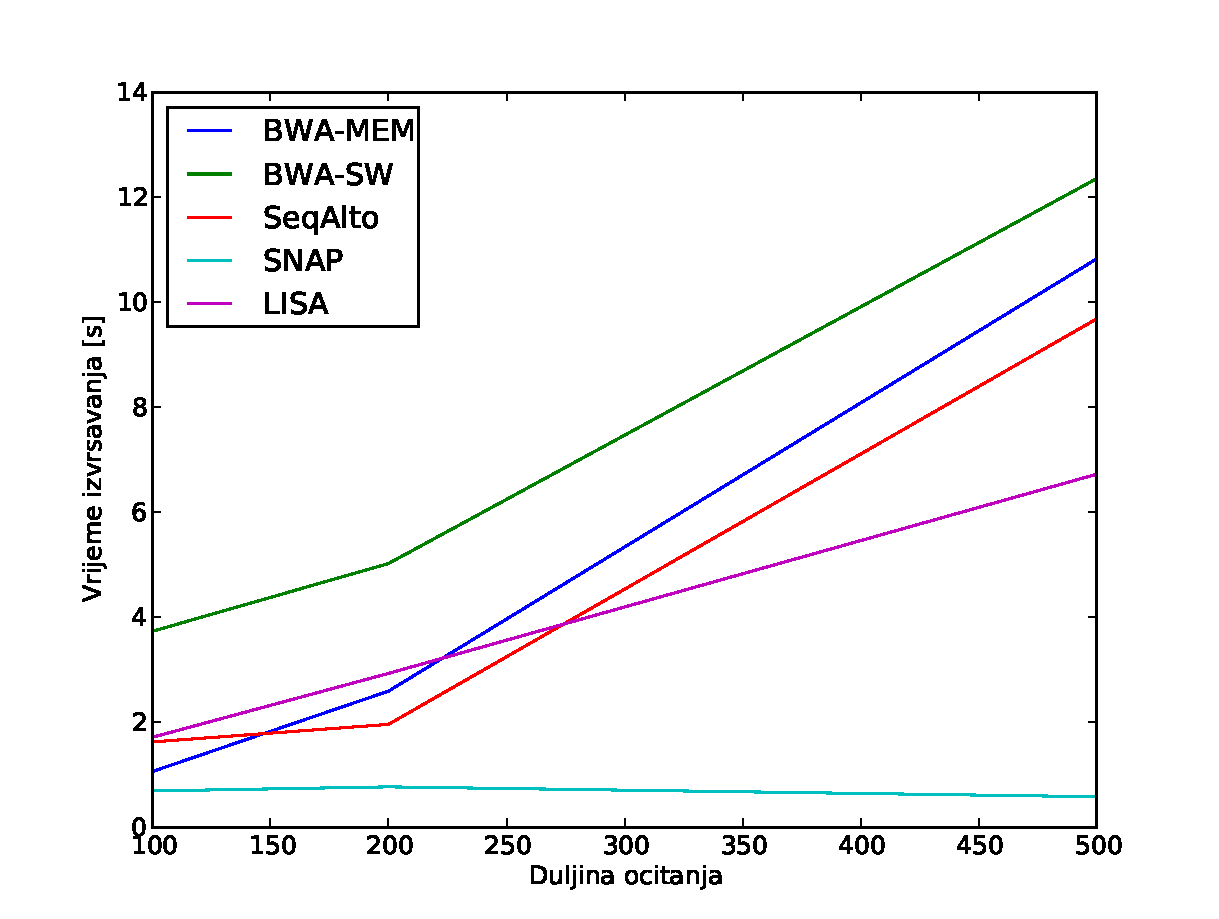
\includegraphics[width=1.0\textwidth]{../img/ecoli-time.pdf}
\caption{Usporedba performansi mappera}
\label{ecoli-time}
\end{figure}

Genom bakterije \emph{E. Coli} sadrži otprilike 5M parova nukleotida. Proveli smo testiranja poravnanja očitanja duljine 100, 200 i 500. Natjecanje vremenskih performansi je jasno pobijedio SNAP (\ref{ecoli-time}). To ne iznenađuje jer je on posebno dizajniran za kraće duljine očitanja. Kasnije ćemo vidjeti da prestaje biti praktičan kada duljine očitanja rastu. LISA performansama nadmašuje preostale mappere. U tablici \ref{ecoli-correct} je vidljivo da su na testiranju svi mapperi bili iznimno precizni.

\begin{table}[H]
\centering
\begin{tabular}{|c||c|c|c|}
\hline
	Duljine & 100 & 200 & 500\\
\hline
\hline
	BWA-MEM & 99.60 & 99.64 & 99.65\\
\hline
	BWA-SW  & 99.55 & 99.64 & 99.65\\
\hline
	SeqAlto & 99.10 & 99.63 & 99.64\\
\hline
	SNAP    & 99.61 & 97.37 & 99.56\\
\hline
	LISA    & 99.54 & 99.63 & 99.62\\
\hline
\end{tabular}
\caption{Postotak točno poravnatih očitanja}\label{ecoli-correct}
\end{table}


\section {Salmonella Enterica}

\begin{figure}[H]
\centering
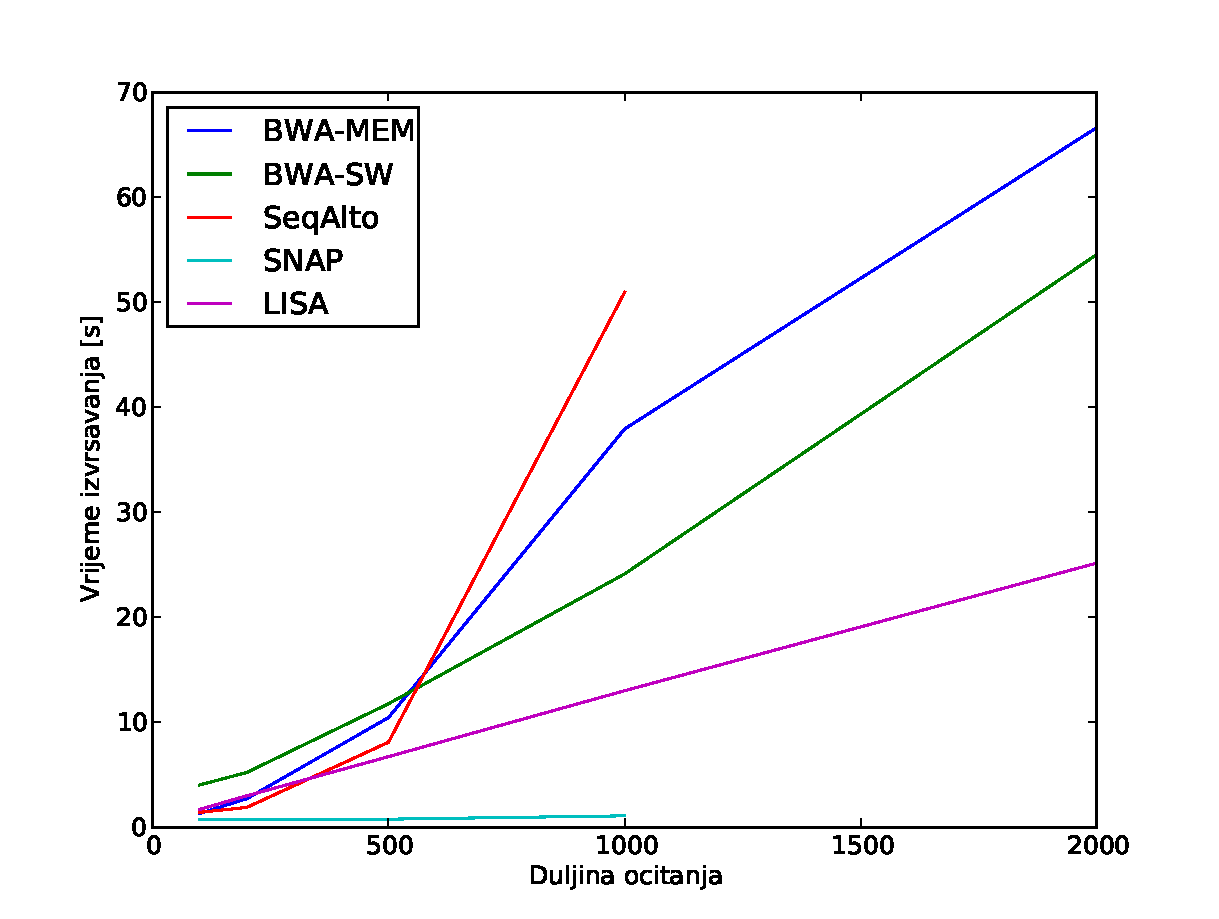
\includegraphics[width=0.97\textwidth]{../img/salmonella-time.pdf}
\caption{Usporedba performansi mappera}\label{salmonella-time}
\end{figure}

Genom \emph{S. Enterica}-e sastoji se od otprilike 5M parova nukoleotida. Proveli smo testiranja poravnanja očitanja duljina 100, 200, 500, 1000 i 2000. Na slici \ref{salmonella-time} je vidljivo da SNAP ima najbolje performanse za očitanja do duljine 1000. Za duljinu 2000 je imao poteškoća sa izvođenje pa nemamo rezultat. Zbog preglednosti grafa izostavili smo rezultat SeqAlto-a na očitanjima duljine 2000 (eksperiment je trajao 6m12s). LISA nadmašuje sve mappere osim SNAP-a na malim duljinama. Tablica \ref{salmonella-correct} ističe iznimnu točnost svih mappera.

\begin{table}[H]
\centering
\begin{tabular}{|c||c|c|c|c|c|}
\hline
	Duljine & 100 & 200 & 500 & 1000 & 2000\\
\hline
\hline
	BWA-MEM & 99.57 & 99.70 & 99.83 & 99.97 & 99.99\\
\hline
	BWA-SW  & 99.53 & 99.69 & 99.82 & 99.97 & 99.99\\
\hline
	SeqAlto & 99.06 & 99.69 & 99.83 & 99.97 & 99.99\\
\hline
	SNAP    & 99.13 & 97.02 & 99.47 & 97.95 & -\\
\hline
	LISA    & 99.54 & 99.67 & 99.81 & 99.95 & 99.91\\
\hline
\end{tabular}
\caption{Postotak točno poravnatih očitanja}\label{salmonella-correct}
\end{table}


\section {Streptococcus Pneumoniae}

\begin{figure}[H]
\centering
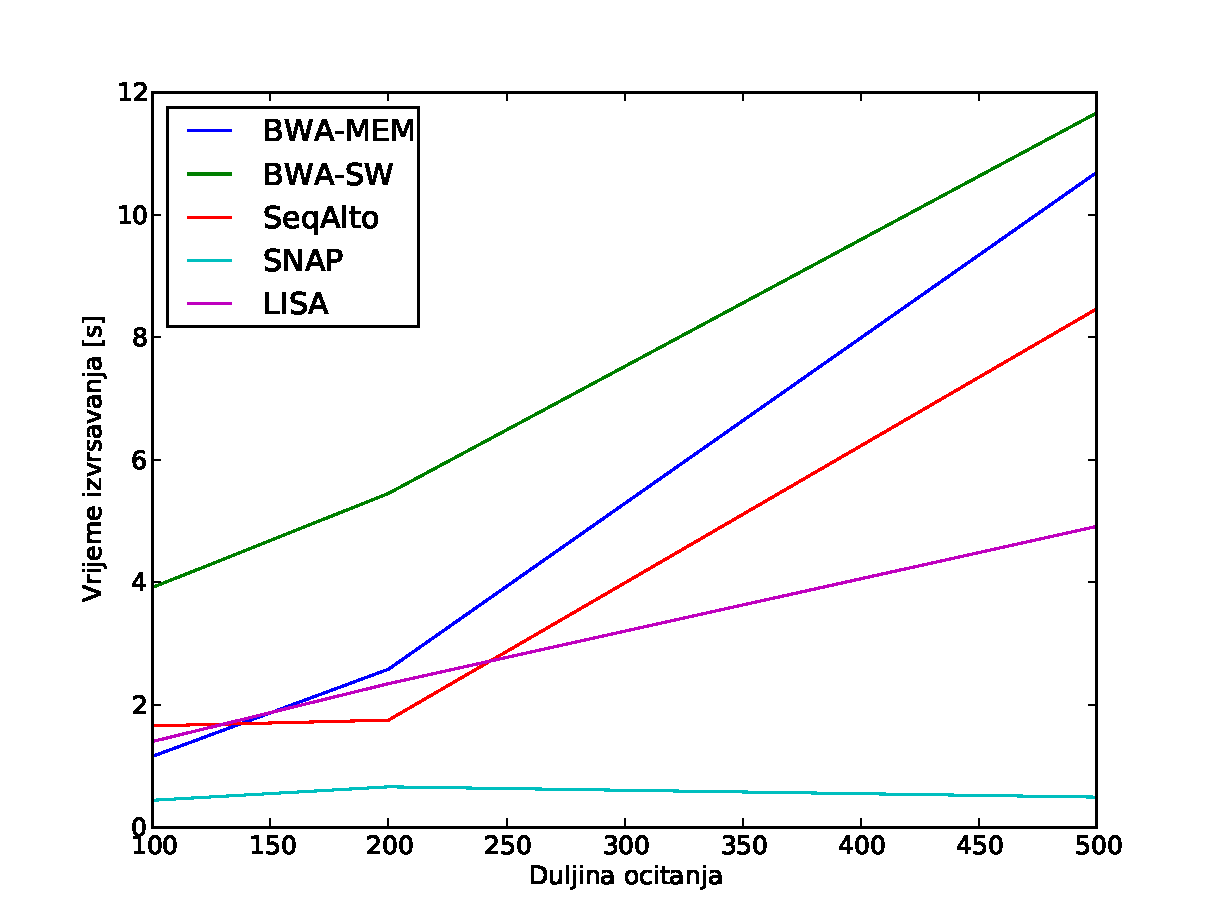
\includegraphics[width=1.0\textwidth]{../img/streptococcus-time.pdf}
\caption{Usporedba performansi mappera}\label{streptococcus-time}
\end{figure}

Genom \emph{S. Pneumoniae} sadrži otprilike 3M parova nukleotida. Proveli smo testiranja poravnanja očitanja duljina 100, 200 i 500. Na slici \ref{streptococcus-time} vidljivo je kako na ovim kraćim duljinama SNAP ima najbolje performanse. To je očekivan rezultat budući da je on pažljivo dizajniran za kratke duljine očitanja. LISA je bolja od preostalih mappera. Tablica \ref{streptococcus-correct} pokazuje vrhunsku preciznost svih mappera. Valja istaknuti kako SNAP ima nešto manju preciznost u usporedbi s ostalim mapperima.

\begin{table}[H]
\centering
\begin{tabular}{|c||c|c|c|}
\hline
	Duljine & 100 & 200 & 500\\
\hline
\hline
	BWA-MEM & 99.10 & 99.38 & 99.55\\
\hline
	BWA-SW  & 99.12 & 99.37 & 99.54\\
\hline
	SeqAlto & 98.57 & 99.31 & 99.52\\
\hline
	SNAP    & 97.74 & 96.26 & 98.82\\
\hline
	LISA    & 98.98 & 99.36 & 99.53\\
\hline
\end{tabular}
\caption{Postotak točno poravnatih očitanja}\label{streptococcus-correct}
\end{table}


\section {Yersinia Pestis}

\begin{figure}[H]
\centering
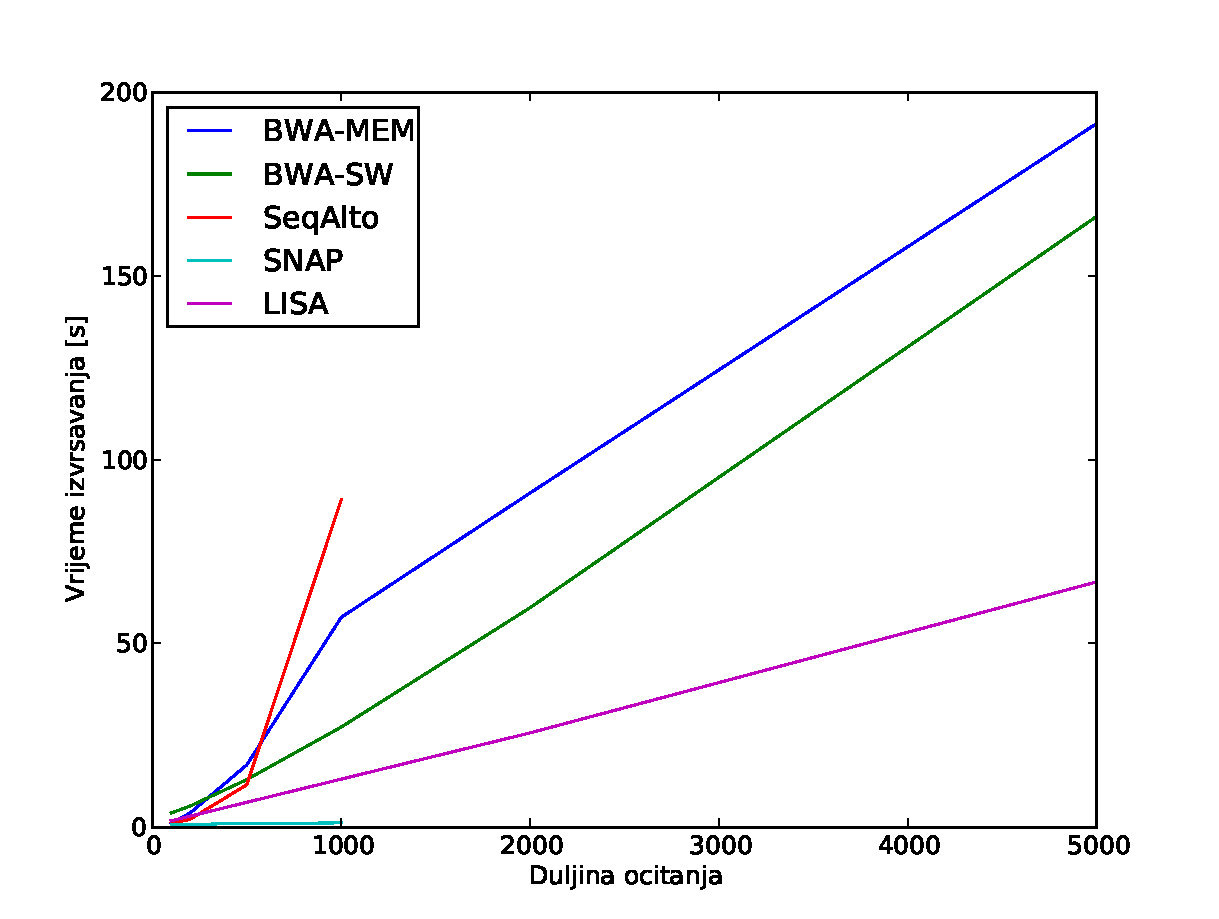
\includegraphics[width=1.0\textwidth]{../img/yersinia-time.pdf}
\caption{Usporedba performansi mappera}\label{yersinia-time}
\end{figure}

Genom \emph{Y. Pestis}, šire poznate kao kuga, sadrži otprilike 5M parova nukleotida. Proveli smo testiranja poravnanja očitanja duljina 100, 200, 500, 1000, 2000 i 5000. Slika \ref{yersinia-time} demonstrira efikasnost SNAP-a na manjim duljinama. SNAP je imao poteškoća s obrađivanjem očitanja duljina većih od 1000, iz tog razloga izostaju ti rezultati. Zbog preglednosti grafa na njemu nisu vidljiva vremena izvođenja SeqAlto-a za duljine 2000 (7m9s) i 5000 (19m27s). Za dugačka očitanja LISA se ponaša uvjerljivo najbolje, postižući ubrzanja 3-20x u usporedbi s ostalim mapperima. Točnosti svih mappera su vidljive u tablici \ref{yersinia-correct}. Svi mapperi su vrlo velike i točnosti zadovoljavajuće za praktičnu uporabu.

\begin{table}[H]
\centering
\begin{tabular}{|c||c|c|c|c|c|c|}
\hline
	Duljine & 100 & 200 & 500 & 1000 & 2000 & 5000\\
\hline
\hline
	BWA-MEM & 95.63 & 96.31 & 97.34 & 98.66 & 99.90 & 100.00\\
\hline
	BWA-SW  & 95.60 & 96.31 & 97.33 & 98.58 & 99.79 & 99.98\\
\hline
	SeqAlto & 95.12 & 96.29 & 97.37 & 98.63 & 99.88 & 63.85\\
\hline
	SNAP    & 96.64 & 93.34 & 96.57 & 96.22 & - & -\\
\hline
	LISA    & 95.53 & 96.21 & 97.21 & 98.54 & 99.72 & 99.81\\
\hline
\end{tabular}
\caption{Postotak točno poravnatih očitanja}\label{yersinia-correct}
\end{table}


\section {Dodatne informacije}
Ovdje navodimo naredbe kojima smo pokretali svaki od mappera.

\begin{table}[H]
\centering
\begin{tabular}{|c|c|}
\hline
BWA-MEM & bwa mem -t 24 index ocitanja.fq > rezultat.sam\\
\hline
BWA-SW & bwa bwasw -t 24 index ocitanja.fq > rezultat.sam\\
\hline
SeqAlto & seqalto\_basic align index -n 1 -f -p 24 ocitanja.fq >rezultat.sam\\
\hline
 & Za duljine < 500: snap single index ocitanja.fq -t 24\\
SNAP & Za duljinu 500: snap single index ocitanja.fq -t 24 -d 20\\
& Za duljinu 1000: snap single index ocitanja.fq -t 24 -d 40 -h 100 -n 2000\\
\hline
LISA & client solve genom.fasta index ocitanja.fq /dev/null\\
\hline
\end{tabular}
\label{komande}
\end{table}


\chapter{Zaključak i daljnji rad}

\section{Osvrt}
U ovom radu prezentirali smo LISA-u, novi alat za poravnanje očitanja na referentni genom. Proveli smo usporedbu s trenutno najpopularnijim alatima i pokazali da LISA već u svojoj ranoj fazi razvoja pokazuje jako dobre performanse, pogotovo za očitanja velike duljine. Duljine očitanja su u trendu porasta tako da predviđamo da će tehnike korištene biti od značaja u bližoj i daljoj budućnosti.

\section{Daljnji rad}
Najveći istraživački prioritet kojem su autori trenutno posvećeni je povećanje točnosti mapiranja očitanja malih duljina kao i onih s velikom greškom. Slutnja koju još valja potvrditi je da zadovoljavajuće točnosti možemo dobiti aproksimiranjem metrika kvalitete koje koriste SNAP ili SeqAlto. Te se metrike mogu aproksimirati s manjom računskom složenosti od izračuna pravih vrijednosti pa vjerujemo da neće biti znatnog gubitka vremenskih performansi.\\
Implementacijski prioritet je ispisivanje rezultata u standardiziranom SAM formatu jer se tada otvara mogućnost korištenja mnogih već razvijenih alata za analizu efikasnosti i rezultata.

\chapter{Dodatak}

\section{Najdulji rastući podniz\cite{Fredman197529}}
\emph{Definicija:} Za zadani niz od $n$ brojeva $a_i$ potrebno je naći najveći podskup indeksa tako da u odabranom podskupu za svako $i < j$ vrijedi $a_i < a_j$.
\\
U ovom poglavlju dani su isječci koda koji jasno i jednostavno implementiraju algoritam koji rješava problem najduljeg rastućeg podniza. U svrhu sažetosti izostavljena je implementacija Fenwickovog stabla. To je stablo klasična struktura i njenu je implementaciju vrlo lako dobaviti. Samo napominjemo da operacije $Fenwick.get(x)$ dobavlja najveći element u intervalu $[1,x]$, dok $Fenwick.update(x, v)$ postavlja vrijednost na indeksu $x$ na vrijednost $v$.


\begin{algorithm}[H]
\begin{lstlisting}

void reconstructLIS(vector<int>* result,
                    int last,
                    const vector<int>& reconstructionTable) {
  result->clear();
  result->reserve(reconstructionTable.size());
  for ( ; last != -1; last = reconstructionTable[last]) {
    result->push_back(last);
  }
  reverse(result->begin(), result->end());
}

\end{lstlisting}
\end{algorithm}


\begin{algorithm}[H]
\begin{lstlisting}
void calcLongestIncreasingSubsequence(
    vector<int>* result,
    const vector<pair<int, int> >& elements) {
  int n = elements.size();

  vector<int> dpTable(n, 0);
  vector<int> reconstructionTable(n, -1);

  int maxSecond = -1;
  for (int i = 0; i < elements.size(); ++i) {
    maxSecond = max(maxSecond, elements[i].second);
  }

  FenwickMax fm(maxSecond);

  for (size_t i = 0; i < n; ++i) {
    std::pair<int, int> best = fm.get(elements[i].second-1);
    if (best.first) {
      dpTable[i] = best.first+1;
      reconstructionTable[i] = best.second;
    } else {
      dpTable[i] = 1;
    }
    fm.update(elements[i].second, make_pair(dpTable[i], i));
  }

  int last = 
        max_element(dpTable.begin(), dpTable.end())-dpTable.begin();
  reconstructLIS(result, last, reconstructionTable);
}
\end{lstlisting}
\end{algorithm}

\nocite{Pabinger21012013}
\nocite{Johnson:2008:BAU:1593105.1593117}

\bibliography{literatura}
\bibliographystyle{plain}

\begin{sazetak}

DNA je struktura koja kodira živi svijet. Bolje razumijevanje funkcija pojedinih dijelova može dovesti do pravovremene detekcije i liječenja mnogih bolesti. Strojevi za očitanje DNA iz dana u dan napreduju i proizvode velike količine sve duljih očitanja. Lociranje očitanja unutar referentnog genoma jedan je od temeljnih otvorenih problema u bioinformatici. U ovom radu predlažemo novi algoritam poravnanja DNA temeljen na brzom traženju najduljeg rastućeg podniza, posebno pogodnim za dulja očitanja. Napravljena je usporedba točnosti i brzine s trenutno najefikasnijim i najpopularnijim alatima.

\kljucnerijeci{poravnavanje DNA, bioinformatika, algoritmi, hash, LISA, najdulji rastući podniz}
\end{sazetak}

\engtitle{LISA - DNA reads alignment tool}
\begin{abstract}
DNA is a structure which encodes all of the living world. Better understanding of it's particular section could lead to detection and curing of many diseases. DNA sequencing machines are getting better every day and producing
big amounts of ever longer reads. Locating these reads inside a reference genome is a fundemental open problem in bioinformatics. This paper presents a novel DNA alignment algorithm, based on a fast longest increasing subsequence search. It is very feasible for long reads. Detailed analysis and comparison with state-of-the-art tools is given.

\keywords{DNA alignment, bioinformatics, algorithms, hash, LISA, longest increasing subsequence}
\end{abstract}

\end{document}
